\documentclass[a4paper]{article}

% Includes packages relevant to Senior Lab

% character set specifications
\usepackage[english]{babel}
\usepackage[utf8]{inputenc}

% increased vertical spacing for tables
\newcommand\topVspace{\rule{0pt}{2.6ex}}      
\newcommand\bottomVspace{\rule[-1.2ex]{0pt}{0pt}} 

% extra unicode characters
\DeclareUnicodeCharacter{3BC}{\(\mu\)}
\DeclareUnicodeCharacter{3C1}{\(\rho\)}
\DeclareUnicodeCharacter{2080}{\(_0\)}
\DeclareUnicodeCharacter{2081}{\(_1\)}
\DeclareUnicodeCharacter{2082}{\(_2\)}
\DeclareUnicodeCharacter{3B5}{\(\epsilon\)}
\DeclareUnicodeCharacter{3B1}{\(\alpha\)}

% SI Units
\usepackage{siunitx}

% extra SI units
\DeclareSIUnit\gauss{G}

% enable scientific notation
\sisetup{scientific-notation = engineering, exponent-to-prefix}

% draw pretty lines
\usepackage{tikz}
\usetikzlibrary{datavisualization}
\usepackage{circuitikz}

% manual tabbing
\setlength{\parindent}{0pt}
\def\qq{\qquad}

% include graphics
\usepackage{graphicx}

% increased control over figure placement
\usepackage{float}

% box answers
\usepackage{tcolorbox}

% enable multiple section levels
\usepackage{titlesec}

% define `\subsubsubsection` command
\titleclass{\subsubsubsection}{straight}[\subsection]
\newcounter{subsubsubsection}[subsubsection]
\renewcommand\thesubsubsubsection{\thesubsubsection.\arabic{subsubsubsection}}
\titleformat{\subsubsubsection}
        {\normalfont\normalsize\bfseries}{\thesubsubsubsection}{1em}{}
\titlespacing*{\subsubsubsection}
{0pt}{3.25ex plus 1ex minus .2ex}{1.5ex plus .2ex}
\setcounter{secnumdepth}{4}

% get align environment (among other things)
\usepackage{amsmath}

% bold in math mode
\usepackage{bm}

% get \mathbb (among other things)
\usepackage{amssymb}

\usepackage{array}

% plotting
\usepackage{pgfplots}

% enable external references
\usepackage{hyperref}

% include code
\usepackage[cache=false]{minted}
\setminted{linenos, frame=lines, texcomments}

% adjust margins of individual pages (for shoving figures into place)
\usepackage{changepage}

% rotate figures
\usepackage{rotating}


\usepackage{caption}
\renewcommand{\thetable}{\arabic{section}.\arabic{table}}
\newcommand\T{\rule{0pt}{2.6ex}}       % Top strut
\newcommand\B{\rule[-1.2ex]{0pt}{0pt}} % Bottom strut

\title{PHY 4210-01 Senior Lab \\Lab P1: Planck's Constant\\Lab P6: Blackbody Radiation}

\author{Sarah Arends \\
        Jacquelyne Miksanek \\
        Ryan Wojtyla \\ \\
        Instructor: Dr. Marcus Hohlmann}

\date{\today}

\begin{document}
\maketitle

\begin{abstract}
%physics of experiment
%apparatus used
%what was measured
%Results
\qq 
\end{abstract}

\newpage

\tableofcontents

\newpage

P1 Planck's Constant Experiment

\newpage

\section{Objective of the Experiment}
%A brief statement on the main purpose of the experiment
\qq 

\section{Theory of the Experiment}


\section{Equipment Utilized}
%List principal pieces of apparatus used by manufacturer, model and
%serial number. When it may be important, list principal
%specifications of certain pieces of equipment (e.g. the focal length
%of an optical system, etc.)

% Description of set-up in prose
\qq 

% List of specs
\begin{itemize}
\item itemName \\
\item itemName \\
\end{itemize}

%Labeled sketch of the experimental setup
\begin{figure}[H]
\centering
% uncomment the line below to add image
%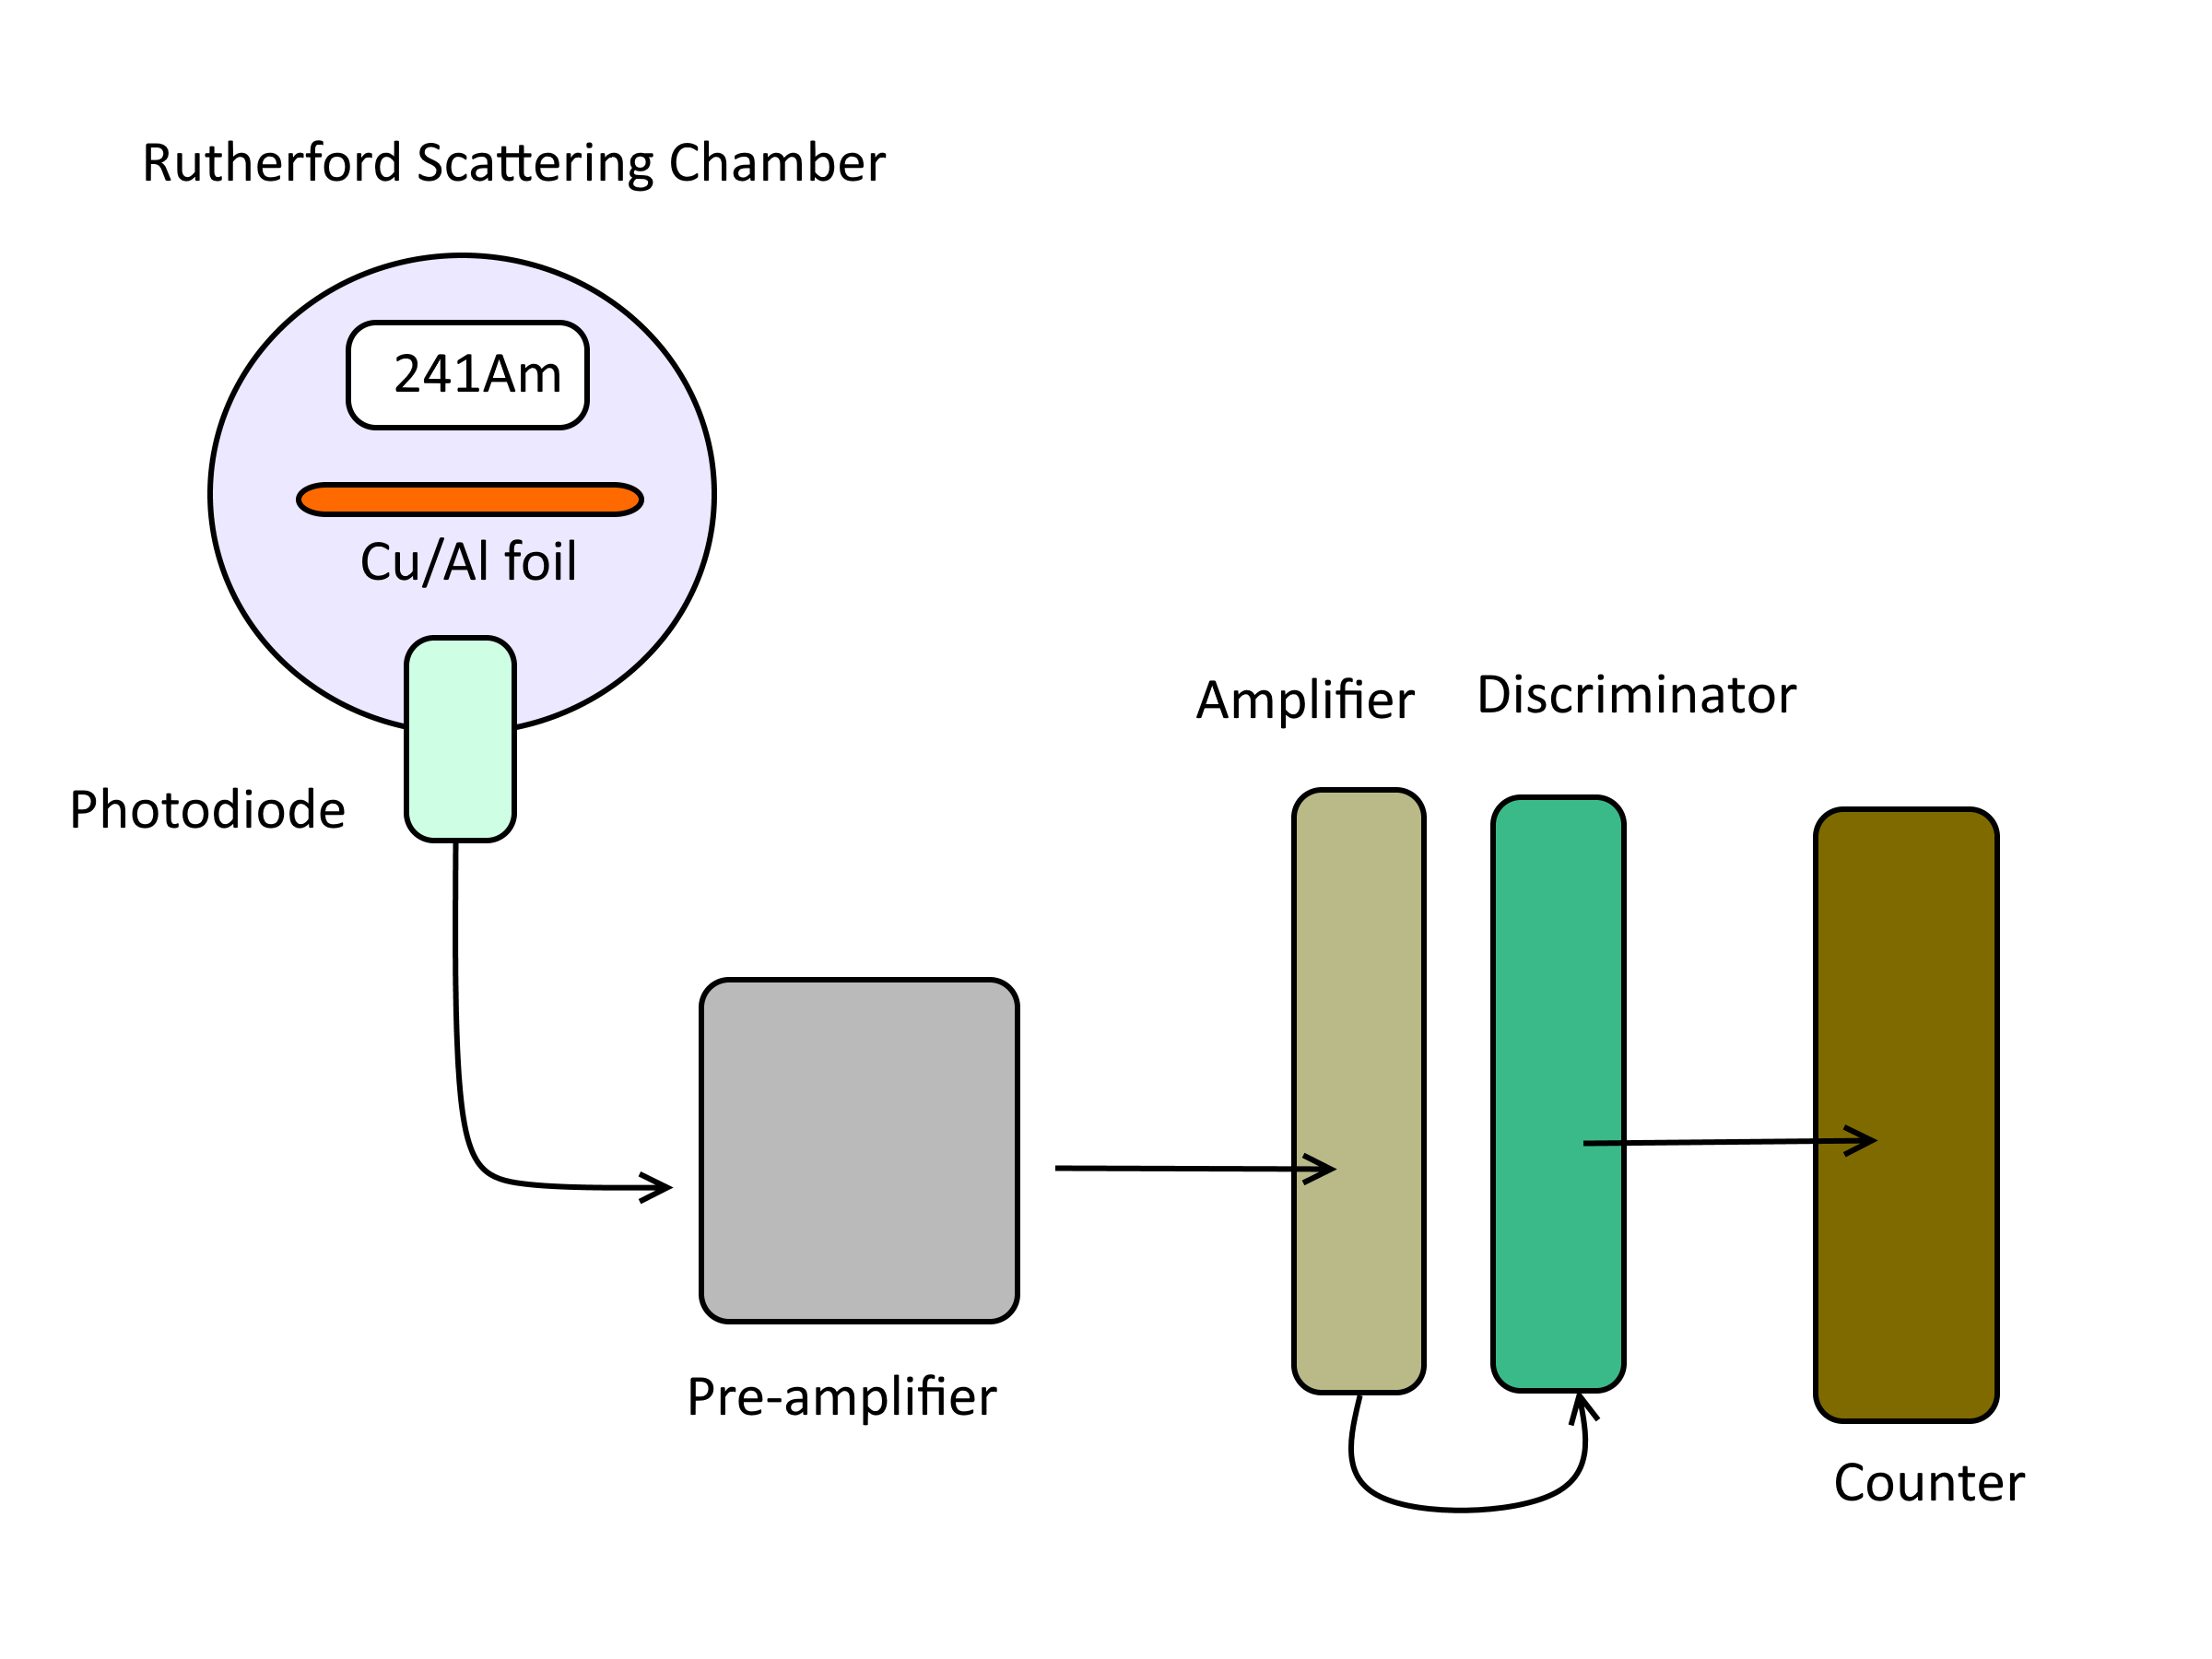
\includegraphics[width=1\textwidth]{diagram.png}
\captionof{figure}{Schematic for circuit diagram }
\label{Diagram}
\end{figure}

\section{Procedure}

% Describe the main steps in the experimental procedures. Be sure to include any
% precautions. Sufficient details should be given such that another student can
% follow and do the experiment.

\subsection{Procedural Modifications}
\qq 

\section{Data Analysis}

%Graphs, figures, and tables with captions
%Results with error analysis
%Calculate discrepancies from theory

\section{Results}

\subsection{Source of Error}

\section{Conclusion}
%Brief summary, discussion of theory

\newpage

P6: Blackbody Radiation

\newpage

\section{Objective of the Experiment}
%A brief statement on the main purpose of the experiment
\qq 

\section{Theory of the Experiment}


\section{Equipment Utilized}
%List principal pieces of apparatus used by manufacturer, model and
%serial number. When it may be important, list principal
%specifications of certain pieces of equipment (e.g. the focal length
%of an optical system, etc.)

% Description of set-up in prose
\qq 

% List of specs
\begin{itemize}
\item itemName \\
\item itemName \\
\end{itemize}

%Labeled sketch of the experimental setup
\begin{figure}[H]
\centering
% uncomment the line below to add image
%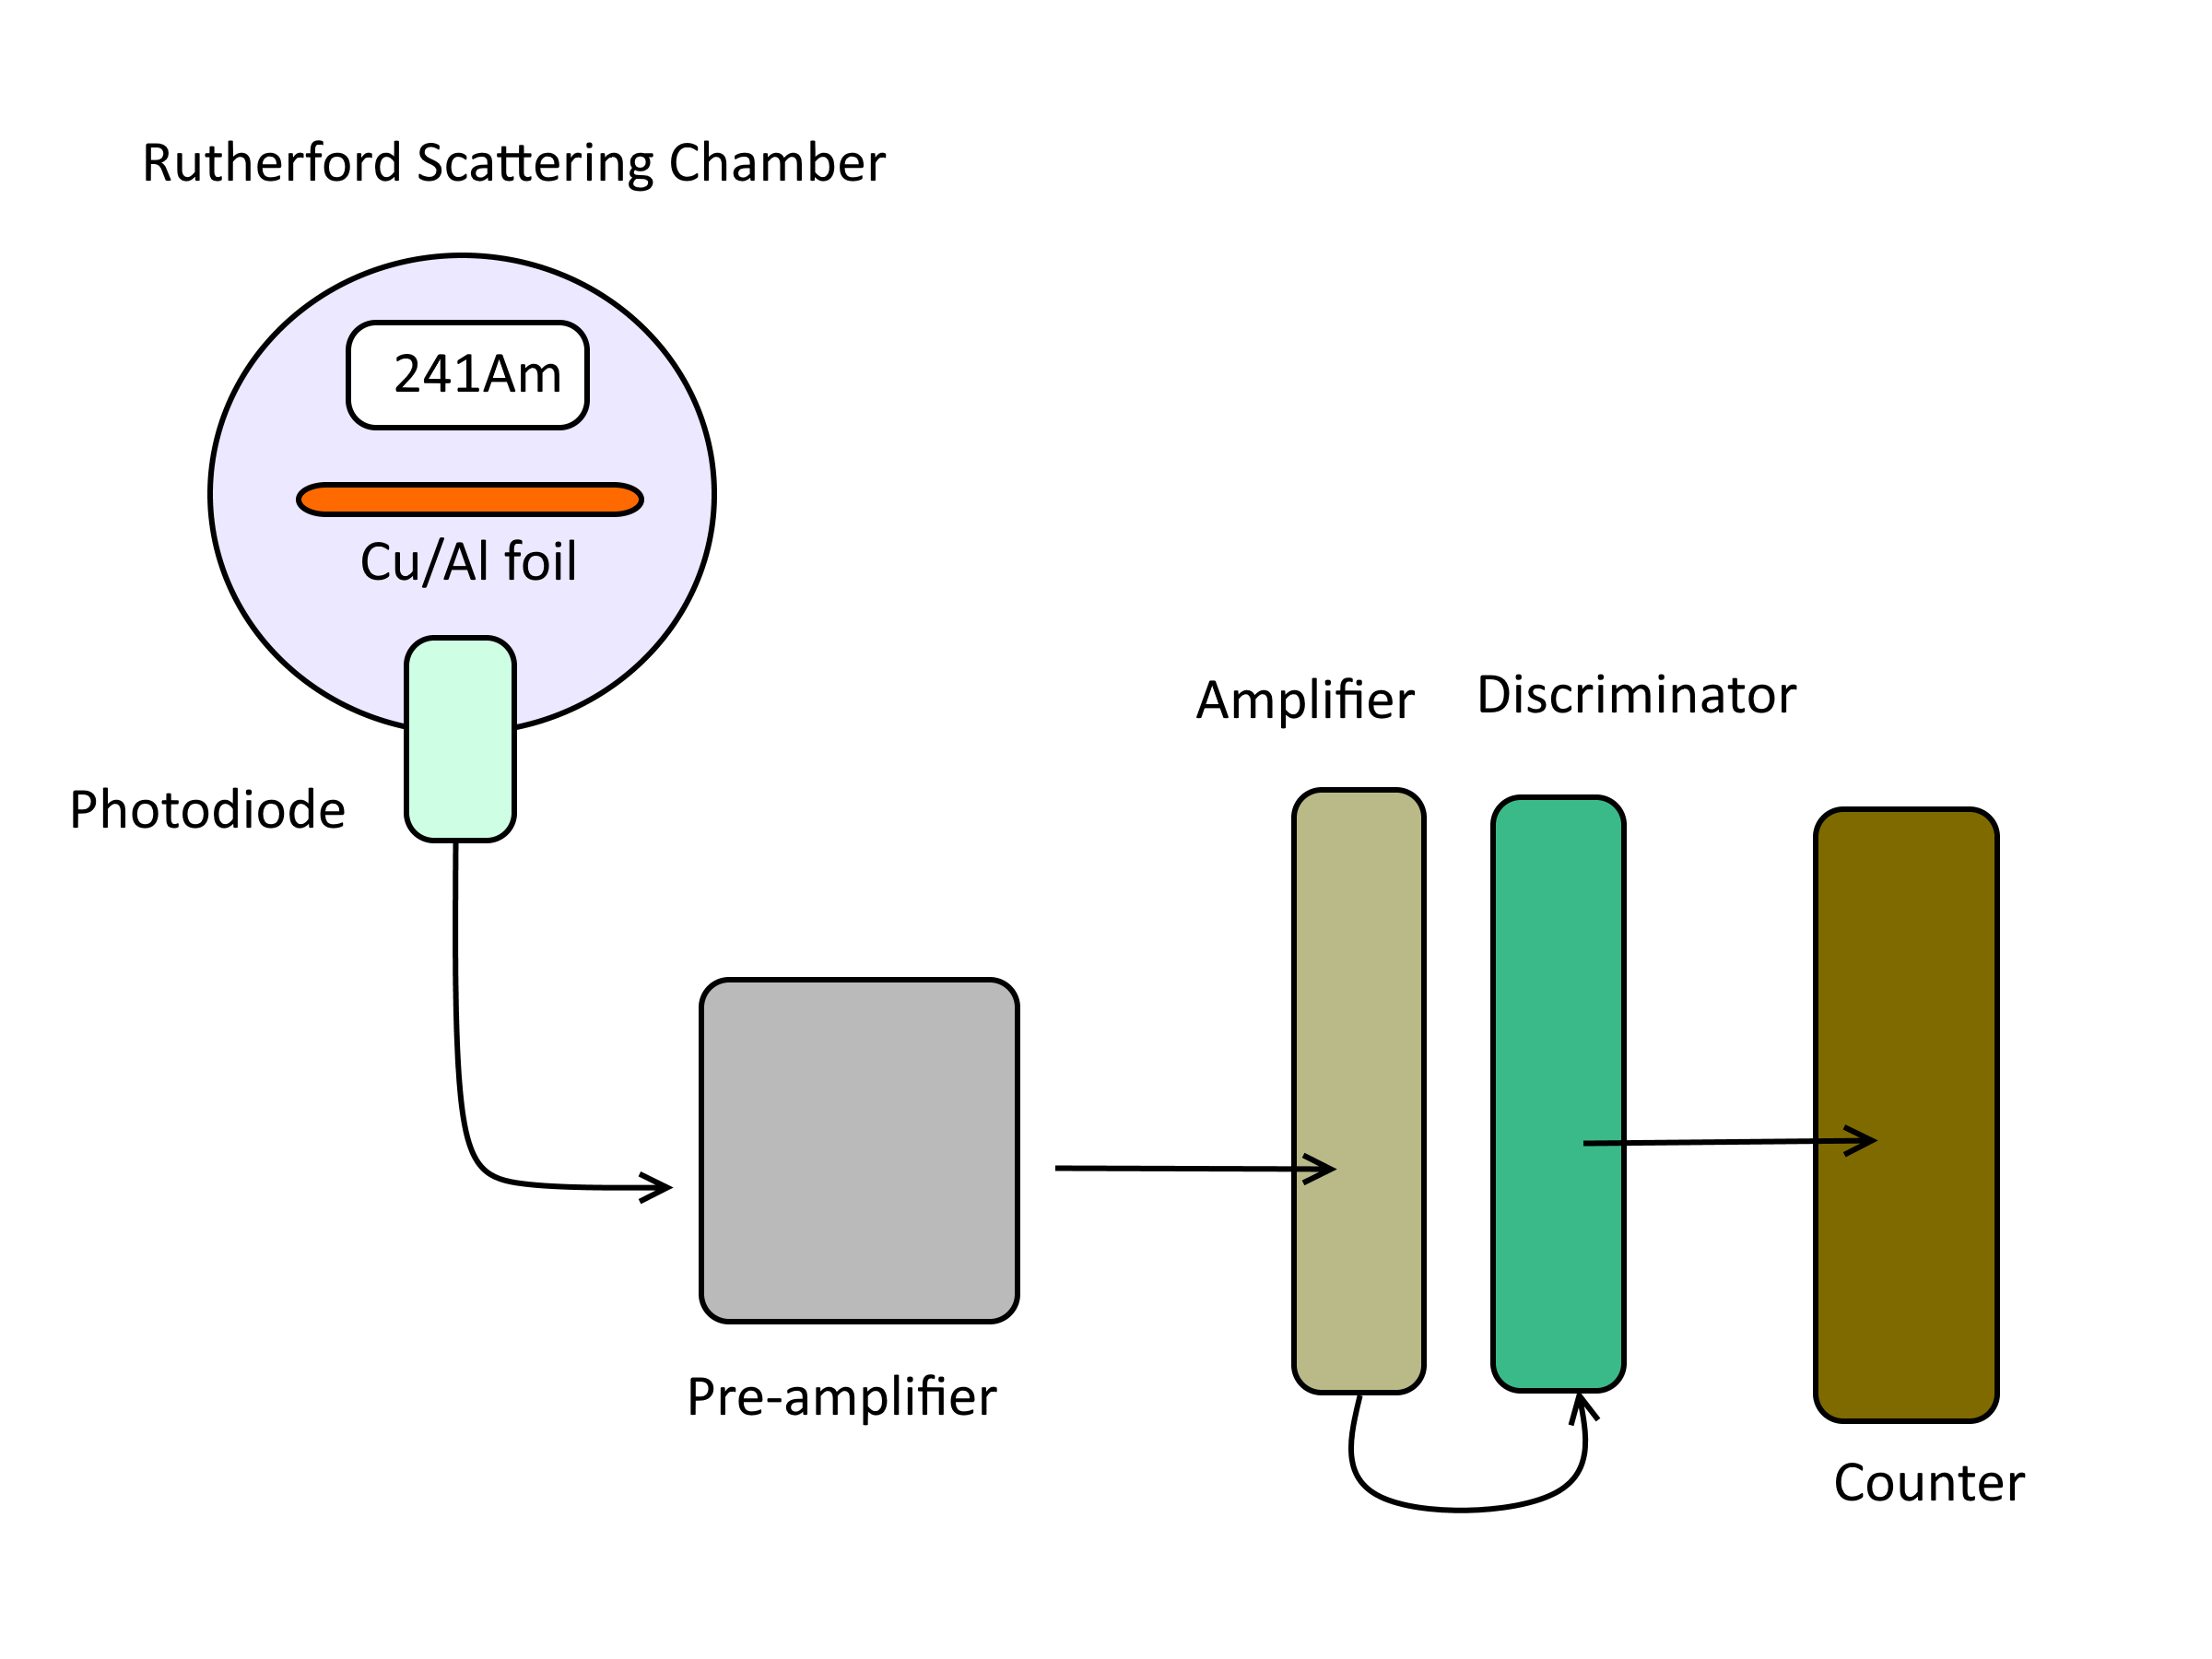
\includegraphics[width=1\textwidth]{diagram.png}
\captionof{figure}{Schematic for circuit diagram }
\label{Diagram}
\end{figure}

\section{Procedure}

% Describe the main steps in the experimental procedures. Be sure to include any
% precautions. Sufficient details should be given such that another student can
% follow and do the experiment.

\subsection{Procedural Modifications}
\qq 

\section{Data Analysis}

%Graphs, figures, and tables with captions
%Results with error analysis
%Calculate discrepancies from theory

\section{Results}

\qq For each of the four voltages, the relative intensity of light incident upon
the broad spectrum light sensor was plotted against the wavelength of the light
being measured by the sensor.

\qq First, \SI{3}{\volt} and \SI{0.388}{\ampere} were applied to the
bulb. Although no clear pattern can be readily discerned from the plot, Figure
\ref{gph:3volt}, at lower wavelengths, a clear peak of intensity occurs at
\( 939 \pm 1 \si{\nano\meter} \). This value is within the range of the
theoretical peak wavelength of \( 1734 \pm 1292 \si{\nano\meter} \). The
discrepancy between the theoretical and experimental values of the peak
wavelength is calculated with
\( \Delta_{\lambda} = | \lambda_t - \lambda_e | \), where \( d \) is the
discrepancy, \( \lambda_t = 939 \pm 1 \si{\nano\meter} \) is the theoretical
value of the peak wavelength, and
\( \lambda_e = 1734 \pm 1292 \si{\nano\meter} \) is the experimental value of
the peak wavelength.

\begin{align*}
  \Delta_{\lambda} =& \left| (939) - (1734) \right| \\
  \Delta_{\lambda} =& 795 \si{\nano\meter} \\
\end{align*}

Since the standard deviation of the wavelengths at \SI{3}{\volt} is \(
\sigma_{\lambda} = \SI{306}{\nano\meter} \), the experimental value of \(
\lambda \) at \SI{3}{\volt} is:

\begin{equation*}
  \frac{\Delta_{\lambda}
\end{equation*}

\subsection{Source of Error}

\section{Conclusion}
%Brief summary, discussion of theory

\section{Appendices}

\end{document}
